\vspace*{1em}

\begin{discussion}[Notation]
Throughout this lecture, we will observe the following notation. Upper case letters $A,\,B,\,C,\ldots,\,X,\,Y,\,Z$ will denote sets, while lower case letters $a,\,b,\,c,\ldots,\,x,\,y,\,z$ will denote elements.\\
\\
We use $\in$ to denote membership of, or belongingness to, a set
\begin{align*}
a \in A:& \text{ ``$a$" \emph{is an element of a set} $A$}\\[0.5em]
a \notin A:& \text{ ``$a$" \emph{is \emph{not} an element of a set} $A$}
\end{align*}
\end{discussion}

\vspace*{1em}

\begin{discussion}[Description of Sets]
There are two ways to describe sets:
\begin{itemize}
\item[(1)] One can list all the elements in a set, enclosing it within \verb!{ }!.
\[A = \set{-4,-2,0,2,4} = \set{0,\pm 2,\pm 4}\]
\item[(2)] Use \emph{set-builder notation}, where we first introduce a general element and the describe the relevant property that defines the set. The recipe is
\[\setp{\text{typical element}}{\text{properties of that element}}\]
The vertical bar is read \emph{such that}; the notation as a whole is to be read as ``those elements such that they have this property''. For example, we can write the set $A$ above as follows; here $\zz$ denotes the set of integers
\begin{align*}
A &= \setp{n \in \zz}{n \text{ is even and }\abs{n} \leq 4}\\[0.5em]
 &= \setp{n \in \zz}{n = 2k, \text{ for some $k \in \zz$, and }\abs{k} \leq 2}.
\end{align*}
So, $A$ is read as ``those integers $n$ \emph{such that} $n$ is even and $\abs{n} \leq 4$''.
\end{itemize}
\end{discussion}

\vspace*{1em}

\begin{definition}[The Empty Set]\label{empty-set}
There is a set with \emph{no elements}, denoted $\emptyset$; we call it the \cdef{empty\ set}.\\[0.5em]
The set can be realised via various descriptions. A mathematical description is the set \[\setp{x \in \zz}{x^2 < 0}.\]
A non-mathematical description is the set of words in the English language that start with the letter \emph{z} and end with the letter \emph{q}.

\begin{dangerbend}
While $\emptyset$ has no elements, the set $X = \set{\emptyset}$ is not the empty set. It is a set with one element -- the empty set, $\emptyset \in X$.
\end{dangerbend}
\end{definition}

\vspace*{1em}

\begin{definition}[Cardinality]\label{cardinality}
The \cdef{cardinality} of a set is the number of elements in the set. For a set $X$, its cardinality is denoted $\card{X}$ or $\abs{X}$.\\[0.5em]
For example, let $A = \set{0,\pm 2,\pm 4}$, then $\card{A} = 5$.

\begin{dangerbend}
The notion of cardinality is clear for finite sets, that is, sets with finitely many elements. We will promptly ignore this notion, for now, for infinite sets. 
\end{dangerbend}
\end{definition}

\vspace*{2em}

\begin{mdframed}
\begin{center}
{\Large Subsets}\label{subsets}
\end{center}
\end{mdframed}

\begin{definition}[Subsets]
Given two sets $S$ and $X$, we say $S$ is a \cdef{subset} of $X$ if every element of $S$ is also an element of $X$, and denote it as $S \subseteq X$. That is, $S$ is the set of \emph{some} elements of $X$.
\[\begin{tikzpicture}[scale=0.85]
	\begin{scope}
	\filldraw[fill=forest,fill opacity=1/5,thick]   (0:0) circle (2);
    \filldraw[fill=green!30!white,thick] (0:-0.5) circle (1);
    \end{scope}
%\draw[thick] (-3,-2.5) rectangle (3,2.5);
\node at (0:1.2)    {$X$};
\node at (0:-0.5)    {$S$};
\end{tikzpicture}\]
Any set $X$ always has two subsets: itself and the empty set.
\end{definition}

\vspace*{1em}

\begin{example}
Let $B = \set{\emptyset,\set{\emptyset},1,2,\set{1,2}}$, then
\begin{align*}
\emptyset \in B,&\ \text{ so } \set{\emptyset} \subseteq B & \set{\emptyset} \in B,&\ \text{ so } \set{\set{\emptyset}} \subseteq B & 1,\,2 \in B,&\ \text{ so } \set{1,2} \subseteq B
\end{align*}
Also, $\set{1,2} \in B$ and $\emptyset,\,B \subseteq B$ as always.

\begin{dangerbend}
This example highlights a common error. We note that $\set{1,2} \subseteq B$ since $1$ and $2$ are \emph{elements} of $B$. But also $\set{1,2} \in B$, since $\set{1,2}$ is also an element of $B$.\\[0.5em]
Being an element means it itself is listed, as is, in a set; while being a subset means \emph{the elements of the subset} are listed as is. For example, take $C = \set{1,2,3}$; then $\set{1,2} \subseteq C$ but $\set{1,2} \notin C$ since the set $\set{1,2}$ is not an element of $C$.
\end{dangerbend}
\end{example}

\vspace*{1em}

We now use the notion of subsets to define what it means for two sets to be equal.
\begin{definition}[Equality of Sets]\label{equality-sets}
We say two sets $A$ and $B$ are equal if $A \subseteq B$ and $B \subseteq A$, and we denote it $A = B$.
\end{definition}

\vspace*{1em}

\begin{definition}[Proper Subsets]
A set $S$ is called a \cdef{proper\ subset} of $X$ if $S \subseteq X$ and $S \neq X$. We denote this as $S \subset X$ or $S \subsetneq X$. In other words, $S$ is a subset that is ``strictly smaller than $X$''.\\[0.5em]
If the set is non-empty, then it has a proper subset -- the empty set.
\end{definition}

\vspace*{1em}

\begin{definition}[Power Set]\label{power-set}
The \cdef{power\ set} of a set $X$ is the set of \emph{all} subsets of $X$, including $X$ and $\emptyset$. We denote it $\mathscr{P}(X)$.\\[0.5em]
For several reasons, the power set is also denoted as $2^X$, one reason is revealed below.
\end{definition}

%\vspace*{1em}

\begin{example}
Let's compute power sets of some sets.
\begin{itemize}[itemsep=0.5em]
\item[(1)] Let $A = \set{1,2,3}$, so $\abs{A} = 3$.
\begin{align*}
\emptyset \subseteq A&\\[0.5em]
1 \in A&, \text{ so } \set{1} \subseteq A\\[0.5em]
1,\,2 \in A&, \text{ so } \set{1,2} \subseteq A\\[0.5em]
1,\,2,\,3 \in A&, \text{ so } A = \set{1,2,3} \subseteq A
\end{align*}
We then get
\[\mathscr{P}(A) = \set{\emptyset,\set{1},\set{2},\set{3},\set{1,2},\set{2,3},\set{1,3},\set{1,2,3}}\]
Note that $\abs{\mathscr{P}(A)} = 8 = 2^3 = 2^{\abs{A}}$.

\item[(2)] Let $A = \set{1,\set{2}}$, so $\abs{A} = 2$. We have
\[\mathscr{P}(A) = \set{\emptyset,\set{1},\set{\set{2}},\set{1,\set{2}}}\]
$\abs{\mathscr{P}(A)} = 4 = 2^2 = 2^{\abs{A}}$.

\item[(3)] Let $A = \emptyset$, so $\abs{A} = 0$. We have
\[B = \mathscr{P}(A) = \set{\emptyset},\quad \abs{\mathscr{P}(A)} = 1 = 2^0 = 2^{\abs{A}}\]
What about $\mathscr{P}(B)$? We have
\[C = \mathscr{P}(B) = \set{\emptyset,\set{\emptyset}}\]
Finally,
\[\mathscr{P}(C) = \set{\emptyset,\set{\emptyset},\set{\set{\emptyset}},\set{\emptyset,\set{\emptyset}}}\]
\end{itemize}

\vspace*{1em}

\begin{remark}
It's true in general that $\abs{\mathscr{P}(X)} = 2^{\abs{X}}$, for any set $X$.
\end{remark}
\end{example}

\vspace*{2em}

\begin{mdframed}
\begin{center}
{\Large Set Operations}\label{set-operations}
\end{center}
\end{mdframed}

We assume all the sets in the section are subsets of some set $U$, labelled the ``universal set''.
\begin{definition}[Set Operations]
Let $A,\,B \subseteq U$.
\begin{itemize}[itemsep=1em]
\item The \cdef{union} of $A$ and $B$ is the set
\[A \cup B = \setp{x \in U}{x \in A \text{ \emph{or} } x \in B}\]
Here our use of ``or'' allows the possibility of $x$ being in both $A$ and $B$.

\item The \cdef{intersection} of $A$ and $B$ is the set
\[A \cap B = \setp{x \in U}{x \in A \text{ \emph{and} } x \in B}\]\newpage
It is clear definitionally that we always have $A \cap B \subseteq A \cup B$.
\[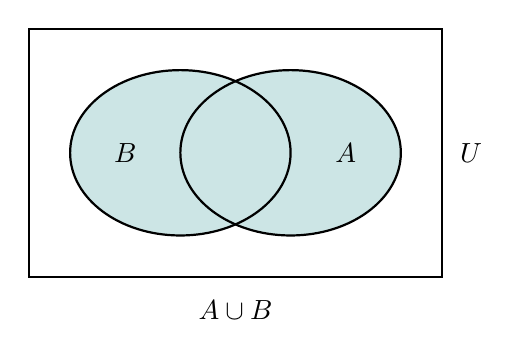
\begin{tikzpicture}[scale=0.7]
	\def\firstcircle{(0:1) ellipse (2cm and 1.5cm)};
    \def\secondcircle{(0:-1) ellipse (2cm and 1.5cm)};
	\begin{scope}
	\fill[white!80!teal] (0:1) ellipse (2cm and 1.5cm);
    \fill[white!80!teal] (0:-1) ellipse (2cm and 1.5cm);
    \end{scope}    
\draw[thick] \firstcircle;
\draw[thick] \secondcircle;
\node at (0:2)    {$A$};
\node at (0:-2)    {$B$};
\draw[thick] (-3.75,-2.25) rectangle (3.75,2.25);
\node[right,xshift=3pt] at (3.75,0){$U$};
\node[below,yshift=-5pt] at (0,-2.25){$A \cup B$};
\end{tikzpicture}\qquad
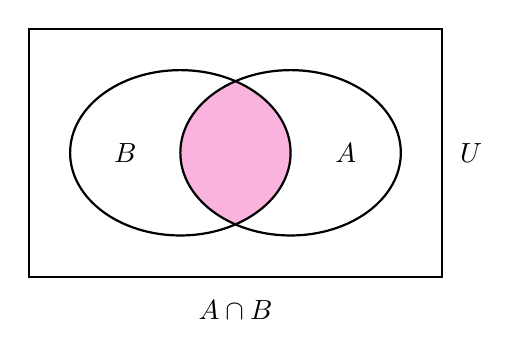
\begin{tikzpicture}[scale=0.7]
	\def\firstcircle{(0:1) ellipse (2cm and 1.5cm)};
    \def\secondcircle{(0:-1) ellipse (2cm and 1.5cm)};
	\begin{scope}
    \clip \firstcircle;
    \fill[white!70!magenta] \secondcircle;
    \end{scope}    
\draw[thick] \firstcircle;
\draw[thick] \secondcircle;
\node at (0:2)    {$A$};
\node at (0:-2)    {$B$};
\draw[thick] (-3.75,-2.25) rectangle (3.75,2.25);
\node[right,xshift=3pt] at (3.75,0){$U$};
\node[below,yshift=-5pt] at (0,-2.25){$A \cap B$};
\end{tikzpicture}\]

\item The \cdef{difference} of $A$ and $B$ is the set
\[A\setminus B = A - B = \setp{x \in U}{x \in A \text{ \emph{and} } x \notin B}\]
That is, it is the set that's left when we remove the part of $B$ that belonged to $A$. Similarly, we can also consider the set that's left when we remove the part of $A$ that belonged to $B$
\[B\setminus A = B - A = \setp{x \in U}{x \in B \text{ \emph{and} } x \notin A}\]
A related operation is the \cdef{symmetric\ difference} defined as
\[A\, \triangle\, B = (A \setminus B) \cup (B \setminus A)\]
\[\begin{tikzpicture}[scale=0.7]
	\def\firstcircle{(0:1) ellipse (2cm and 1.5cm)};
    \def\secondcircle{(0:-1) ellipse (2cm and 1.5cm)};
    	\begin{scope}[even odd rule]
    		\clip \secondcircle (-2,-2) rectangle (3,3);
    		\fill[firebrick!50!white] \firstcircle;
	\end{scope}
\draw[thick] \firstcircle;
\draw[thick] \secondcircle;
\node at ( 0:2)    {$A$};
\node at (0:-2)    {$B$};
\draw[thick] (-3.75,-2.25) rectangle (3.75,2.25);
\node[right,xshift=3pt] at (3.75,0){$U$};
\node[below,yshift=-5pt] at (0,-2.25){$A \setminus B$};
\end{tikzpicture} \qquad
\begin{tikzpicture}[scale=0.7]
	\def\firstcircle{(0:1) ellipse (2cm and 1.5cm)};
    \def\secondcircle{(0:-1) ellipse (2cm and 1.5cm)};
    	\begin{scope}[even odd rule]
    		\clip \firstcircle (2,-2) rectangle (-3,3);
    		\fill[newblue!50!white] \secondcircle;
	\end{scope}
\draw[thick] \secondcircle;
\draw[thick] \firstcircle;
\node at ( 0:2)    {$A$};
\node at (0:-2)    {$B$};
\draw[thick] (-3.75,-2.25) rectangle (3.75,2.25);
\node[right,xshift=3pt] at (3.75,0){$U$};
\node[below,yshift=-5pt] at (0,-2.25){$B \setminus A$};
\end{tikzpicture}\]
\[\begin{tikzpicture}[scale=0.7]
	\def\firstcircle{(0:1) ellipse (2cm and 1.5cm)};
    \def\secondcircle{(0:-1) ellipse (2cm and 1.5cm)};
	\begin{scope}[even odd rule]
    		\clip \secondcircle (-2,-2) rectangle (3,3);
    		\fill[white!70!indigo] \firstcircle;
	\end{scope}  
	\begin{scope}[even odd rule]
    		\clip \firstcircle (2,-2) rectangle (-3,3);
    		\fill[white!70!indigo] \secondcircle;
	\end{scope}
\draw[thick] \firstcircle;
\draw[thick] \secondcircle;
\node at ( 0:2)    {$A$};
\node at (0:-2)    {$B$};
\draw[thick] (-3.75,-2.25) rectangle (3.75,2.25);
\node[right,xshift=3pt] at (3.75,0){$U$};
\node[below,yshift=-5pt] at (0,-2.25){$A\, \triangle\, B$};
\end{tikzpicture}\]

\item The \cdef{complement} of $A$ in $U$ is the set \[A^c = \overline{A} = \setp{x \in U}{x \notin A}\]
That is, it is the set of exactly those elements in $U$ that don't belong to $A$.
\[\begin{tikzpicture}[scale=0.7]
	\def\firstcircle{(0:1) ellipse (2cm and 1.5cm)};
\filldraw[fill=white!80!dirt,thick] (-3.75,-2.25) rectangle (3.75,2.25);
\filldraw[fill=white,thick] \firstcircle;
\node at (0:1)    {$A$};
\node[right,xshift=3pt] at (3.75,0){$U$};
\node[below,yshift=-5pt] at (0,-2.25){$A^c$};
\end{tikzpicture}\]
\end{itemize}
\end{definition}

\vspace*{1em}

\begin{proposition}\label{prop:set-id}
We have the following identities
\begin{itemize}
\item[(1)] $A \setminus B = A \cap B^c$
\item[(2)] $(A \cap B)^c = A^c \cup B^c$
\item[(3)] $(A \cup B)^c = A^c \cap B^c$
\end{itemize}
\end{proposition}
\begin{proof}
We give a ``proof by diagram'' for (1)

\begin{minipage}{0.5\textwidth}
\[\begin{tikzpicture}[scale=0.7]
\filldraw[fill=newblue,fill opacity=1/5,thick] (-3.75,-2.25) rectangle (3.75,2.25);
	\def\firstcircle{(0:1) ellipse (2cm and 1.5cm)};
    \def\secondcircle{(0:-1) ellipse (2cm and 1.5cm)};
\filldraw[fill=white,thick] \secondcircle;
\filldraw[fill=firebrick,fill opacity=1/5,thick] \firstcircle;
\node at (0:0.5)    {$A$};
\node[above,yshift=2em] at (0:-3)    {$B^c$};
\node[left,xshift=-3pt] at (-3.75,0){$U$};
\node[below,yshift=-5pt] at (0,-2.25){$A \cap B^c$};
\end{tikzpicture}\]
\end{minipage}$=$
\begin{minipage}{0.5\textwidth}
\[\begin{tikzpicture}[scale=0.7]
	\def\firstcircle{(0:1) ellipse (2cm and 1.5cm)};
    \def\secondcircle{(0:-1) ellipse (2cm and 1.5cm)};
    	\begin{scope}[even odd rule]
    		\clip \secondcircle (-2,-2) rectangle (3,3);
    		\fill[indigo,opacity=1/5] \firstcircle;
	\end{scope}
\draw[thick] \firstcircle;
\draw[thick] \secondcircle;
\node at ( 0:2)    {$A$};
\node at (0:-2)    {$B$};
\draw[thick] (-3.75,-2.25) rectangle (3.75,2.25);
\node[right,xshift=3pt] at (3.75,0){$U$};
\node[below,yshift=-5pt] at (0,-2.25){$A \setminus B$};
\end{tikzpicture}\]
\end{minipage}
Try proving (2) and (3) similarly. Such diagrams are called \emph{Venn diagrams}. We will revisit (2) and (3) when we discuss \emph{de Morgan Laws}.
\end{proof}

\vspace*{2em}

\begin{mdframed}
\begin{center}
{\Large Indexed Collection of Sets}\label{indexed-collection}
\end{center}
\end{mdframed}

\begin{discussion}
For a finite collection of sets
\[\set{A_1,A_2,\ldots,A_n} = \set{A_i}_{i=1}^n = \set{A_i}_{i \in I},\; I = \set{1,2,\ldots,n}\]
we have
\begin{align*}
A_1 \cap A_2 \cap \cdots \cap A_n &= \bigcap_{i=1}^nA_i = \bigcap_{i\in I} A_i\\[0.5em]
A_1 \cup A_2 \cup \cdots \cup A_n &= \bigcup_{i=1}^nA_i = \bigcup_{i\in I} A_i
\end{align*}
That motivates us to consider an arbitrary collection of sets, indexed by an index set $I$.
\begin{align*}
\set{X_\alpha,A_\beta,A_\gamma,\ldots} &= \set{X_\alpha}_{\alpha \in I},\; I = \set{\alpha,\beta,\gamma,\ldots}\\[0.5em]
X_\alpha \cap X_\beta \cap X_\gamma \cap \cdots &= \bigcap_{\alpha \in I} X_\alpha\\[0.5em]
X_\alpha \cup X_\beta \cup X_\gamma \cup \cdots &= \bigcup_{\alpha \in I} X_\alpha
\end{align*}
Our set $I$ has no restrictions; in particular, it is allowed to infinite.
\end{discussion}

\vspace*{1em}

\begin{example}
Let our index set be $I = [1,\infty)$. For each $r \in I$, we consider the set
%\[X_r = \left(-\frac{1}{r},\frac{1}{r}\right)\]
\[\begin{tikzpicture}
    \draw[<->,thick] (-2.75,0)--(2.75,0);
    \begin{scope}
        \draw[thick,firebrick] (-1.75,0)--(1.75,0);
%        \node[label=above:{$1/r$}](A) at (1.75,0) {};
%        \node[label=above:{$-1/r$}](B) at (-1.75,0) {};
		\fill[firebrick] (-1.75,0) circle (2pt);
		\fill[white] (-1.75,0) circle (1.5pt);
		\fill[firebrick] (1.75,0) circle (2pt);
		\fill[white] (1.75,0) circle (1.5pt);
		\fill[black] (2.25,0) circle (1.75pt);
		\fill[black] (-2.25,0) circle (1.75pt);
		\fill[black] (0,0) circle (1.75pt);
        \node[label=above:{$1$}](C) at (2.25,0) {};
        \node[label=above:{$-1$},xshift=-5pt](D) at (-2.25,0) {};
        \node[label=above:{$0$}](E) at (0,0) {};
        \draw [decorate,decoration={brace,amplitude=10pt,mirror,raise=4pt},yshift=0pt,thick]
(-1.75,0) -- (1.75,0) node [black,midway,below,yshift=-1.5em] {$\color{firebrick}X_r$};
        \node[label={$X_r = \left(-\dfrac{1}{r},\dfrac{1}{r}\right)$},yshift=-2.25em](F) at (-6,0) {};
    \end{scope}
\end{tikzpicture}\]
Then one can show that
\begin{align*}
\bigcap_{r \in I}X_r &= \set{0},\; \text{one point set}\\[0.5em]
\bigcup_{r \in I}X_r &= X_1 = (-1,1)
\end{align*}
\end{example}

\vspace*{2em}

\begin{mdframed}
\begin{center}
{\Large Partition of Sets}\label{partition}
\end{center}
\end{mdframed}

Let $A$ be a set, and $\mathscr{S} = \set{X_\alpha}_{\alpha \in I}$ a collection (or family) of non-empty subsets of $A$, where $I$ is some index set. That is, $\emptyset \neq X_\alpha \subseteq A$.

\begin{definition}[Partitions]
A collection $\mathscr{S}$ of subsets of $A$ is said to be a \cdef{partition} of $A$ if
\begin{itemize}
\item[(1)] $X_\alpha \cap X_\beta = \emptyset$ if $\alpha \neq \beta$ (we say $X_\alpha$ and $X_\beta$ are {\color{blue} (\cdef{mutually}) \cdef{disjoint}}); and
\item[(2)] $\bigcup_{\alpha \in I} X_\alpha = A$.
\end{itemize}
\begin{center}
\begin{minipage}{0.4\textwidth}
\[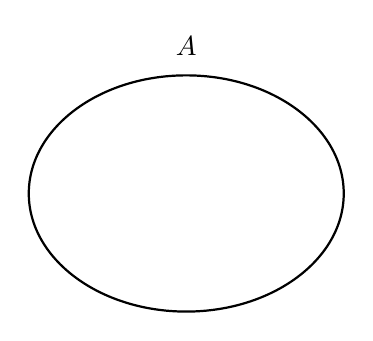
\begin{tikzpicture}
	\node[label=above:{$A$}](A) at (0,1.5) {};	
	\draw[thick] (0,0) ellipse (2cm and 1.5cm);
\end{tikzpicture}\]
\end{minipage}$\overset{\text{partition}}{\underset{\text{of $A$}}{\leadsto}}$
\begin{minipage}{0.4\textwidth}
\[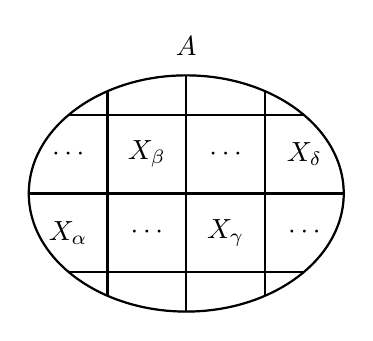
\begin{tikzpicture}
	\node[label=above:{$A$}](A) at (0,1.5) {};	
	\draw[thick] (0,0) ellipse (2cm and 1.5cm);
	\clip[draw] (0,0) ellipse (2cm and 1.5cm);
	\draw[thick] (-2,-2) grid (2,2);
	\node at (-1.5,-0.5) {$X_\alpha$};
	\node at (-0.5,+0.5) {$X_\beta$};
	\node at (+0.5,-0.5) {$X_\gamma$};
	\node at (+1.5,+0.5) {$X_\delta$};
	\node at (+0.5,+0.5) {$\cdots$};
	\node at (-0.5,-0.5) {$\cdots$};
	\node at (-1.5,+0.5) {$\cdots$};
	\node at (+1.5,-0.5) {$\cdots$};
\end{tikzpicture}\]
\end{minipage}
\end{center}

\vspace*{1em}

\begin{remark}
Later we will discuss the notion of ``equivalence relations'' and ``equivalence classes''. Partition of sets play an important role in this context.
\end{remark}
\end{definition}

%\vspace*{1em}

\begin{example}\label{example:modularith}\hfill
\begin{itemize}[itemsep=1em]
\item Let $A = \rr$ be the set of real numbers, we will produce a partition of $\rr$. For any integer $m$, consider the subset $X_m = [m,m+1)$ of $\rr$.
\[\begin{tikzpicture}
    \draw[thick] (-4,0)--(-3.75,0);
    \draw[->,thick,dashed] (-4,0)--(-5,0);
    \draw[->,thick,dashed] (4,0)--(5,0);
	\fill[firebrick] (-3.75,0) circle (1.75pt);
	\draw[thick,firebrick] (-3.75,0)--(-2.5,0);
	\fill[newblue] (-2.5,0) circle (1.75pt);
	\draw[thick,newblue] (-2.5,0)--(-1.25,0);
	\fill[indigo] (-1.25,0) circle (1.75pt);
	\draw[thick,indigo] (-1.25,0)--(0,0);
	\fill[teal] (0,0) circle (1.75pt);
	\draw[thick,teal] (0,0)--(1.25,0);
	\fill[dirt] (1.25,0) circle (1.75pt);
	\draw[thick,dirt] (1.25,0)--(2.5,0);
	\fill[forest] (2.5,0) circle (1.75pt);
	\draw[thick,forest] (2.5,0)--(3.75,0);
	\fill[orange] (3.75,0) circle (1.75pt);
	\draw[thick,orange] (3.75,0)--(4,0);

	\node[label=above:{$1$}] at (1.25,0) {};
	\node[label=above:{$2$}] at (2.5,0) {};
	\node[label=above:{$3$}] at (3.75,0) {};
	\node[label=above:{$-1$},xshift=-5pt] at (-1.25,0) {};
	\node[label=above:{$-2$},xshift=-5pt] at (-2.5,0) {};
	\node[label=above:{$-3$},xshift=-5pt] at (-3.75,0) {};
	\node[label=above:{$0$}] at (0,0) {};

	\node[label=below:{\color{firebrick}\footnotesize $X_{-3}$}] at (-3.125,0) {};
	\node[label=below:{\color{newblue}\footnotesize $X_{-2}$}] at (-1.875,0) {};
	\node[label=below:{\color{indigo}\footnotesize $X_{-1}$}] at (-0.625,0) {};
	\node[label=below:{\color{teal}\footnotesize $X_{0}$}] at (0.625,0) {};
	\node[label=below:{\color{dirt}\footnotesize $X_{1}$}] at (1.875,0) {};
	\node[label=below:{\color{forest}\footnotesize $X_{2}$}] at (3.125,0) {};
\end{tikzpicture}\]
Observe that
\[\begin{cases}
X_m \cap X_k = \emptyset, \text{ for any pair of integers $m \neq k$};\ \text{ and}\\[1em]
\rr = \bigcup_{m \in \zz}X_m\\[0.1em]
\end{cases}\]
Thus, $\setp{X_m}{m \in \zz}$ is a partition of $\rr$

\item Let $A = \zz$ be the set of integers, and let us also choose a positive integer $n$. We will produce a partition of $\zz$ with respect to $n$.\\[0.5em]
For an integer $r$ such that $0 \leq r < n$, consider the following subset of $\zz$
\begin{align*}
[r]_n &= \setp{k \in \zz}{\text{$k$ has remainder $r$ when divided by $n$}}\\[0.5em]
 &= \set{\ldots,-n + r,\,r,\,n + r,\,2n + r,\,3n + r,\ldots}\\[0.5em]
 &= \setp{k \in \zz}{k\equiv r \modar{n}}
\end{align*}
$[r]_n$ is an example of a \emph{congruence class modulo $n$}. Here for two integers $a,\,b \in \zz$ we say $a \equiv b \modar{n}$, ``$a$ is congruent to $b$ modulo $n$'', if $n$ divides $b - a$, written $n \mid (b-a)$.\\[0.5em]
For $n = 3,\ r = 0,1,2$
\begin{align*}
[0]_3 &= \set{\ldots,-6,-3,\,0,\,3,\,6,\,9,\ldots}\\[0.5em]
[1]_3 &= \set{\ldots,-5,-2,\,1,\,4,\,7,\,10,\ldots}\\[0.5em]
[2]_3 &= \set{\ldots,-4,-1,\,2,\,5,\,8,\,11,\ldots}
\end{align*}
Note that the remainder is always positive, for example $-4 = 3(-2) + 2$, which is why $-4 \in [2]_3$. Observe that
\[\begin{cases}
[0]_3 \cap [1]_3 = \emptyset,\;[0]_3 \cap [2]_3 = \emptyset,\;[1]_3 \cap [2]_3 = \emptyset;\ \text{ and}\\[1em]
[0]_3 \cup [1]_3 \cup [2]_3 = \zz\\[0.1em]
\end{cases}\]
Thus, $\set{[0]_3, [1]_3, [2]_3}$ is a partition of $\zz$.
\end{itemize}
We will revisit these example in greater detail later in the course.
\end{example}

\vspace*{2em}

\begin{mdframed}
\begin{center}
{\Large Cartesian Product}
\end{center}
\end{mdframed}

\begin{definition}[Cartesian Product]
For sets $A$ and $B$, we define the \cdef{cartesian\ product} $A \times B$ as the set of ordered pairs
\[A \times B = \setp{(a,b)}{a \in A,\ b \in B}\]
\end{definition}

%\vspace*{1em}

\begin{example}\hfill
\begin{itemize}[itemsep = 1em]
\item[(1)] Let $A = B = \rr$, the set of all real numbers.
\[\rr \times \rr = \setp{(x,y)}{x,\,y \in \rr}\]
Standard notation for this set is $\rr^2$, the Euclidean (or Cartesian) plane.

\item[(2)] $\rr \times \rr \times \rr = \setp{(x,y,z)}{x,\,y,\,z \in \rr}$. Standard notation for this set is $\rr^3$, the three-dimensional Euclidean space.

\item[(3)] Suppose $A = \set{1,2,3}$ and $B = \set{\text{red},\text{blue}}$, then
\[A \times B = \set{(1,\text{red}),(1,\text{blue}),(2,\text{red}),(2,\text{blue}),(3,\text{red}),(3,\text{blue})}\]
\end{itemize}
\end{example}

\vspace*{1em}

\begin{lemma}
$\abs{A \times B} = \abs{A}\cdot \abs{B}$ if both $A$ and $B$ are finite sets.
\end{lemma}
Things quickly get more subtle if $A$ and $B$ were infinite. 

\vspace*{1em}

\begin{remark}
If $A$ and $B$ are disjoint finite sets, that is, $A \cap B = \emptyset$, then
\[\abs{A \cup B} = \abs{A} + \abs{B}\]
But if $A$ or $B$ have infinitely many elements, strange phenomena can occur. For example, consider $A = \nn = \set{1,2,3,\ldots}$, the set of all positive integers, and $B = \set{0}$. Now $A$ is an infinite set, so let's say $\abs{A} = \infty$, and we of course have $\abs{B} = 1$.\\[0.5em]
Note that $A \cap B = \emptyset$, so we expect $\abs{A \cup B} = \abs{A} + \abs{B} = \infty + 1$. What is ``$\infty + 1$''? Does this make sense? We will develop the mathematical theory of infinity later in the course if we have time.
\end{remark}